\section{راهکار پیشنهادی}
\label{sec:solution}
لورم ایپسوم متن ساختگی با تولید سادگی نامفهوم از صنعت چاپ و با استفاده از طراحان گرافیک است. چاپگرها و متون بلکه روزنامه و مجله در ستون و سطرآنچنان که لازم است و برای شرایط فعلی تکنولوژی مورد نیاز و کاربردهای متنوع با هدف بهبود ابزارهای کاربردی می باشد. کتابهای زیادی در شصت و سه درصد گذشته، حال و آینده شناخت فراوان جامعه و متخصصان را می طلبد تا با نرم افزارها شناخت بیشتری را برای طراحان رایانه ای علی الخصوص طراحان خلاقی و فرهنگ پیشرو در زبان فارسی ایجاد کرد. در این صورت می توان امید داشت که تمام و دشواری موجود در ارائه راهکارها و شرایط سخت تایپ به پایان رسد وزمان مورد نیاز شامل حروفچینی دستاوردهای اصلی و جوابگوی سوالات پیوسته اهل دنیای موجود طراحی اساسا مورد استفاده قرار گیرد.

لورم ایپسوم متن ساختگی با تولید سادگی نامفهوم از صنعت چاپ و با استفاده از طراحان گرافیک است. چاپگرها و متون بلکه روزنامه و مجله در ستون و سطرآنچنان که لازم است و برای شرایط فعلی تکنولوژی مورد نیاز و کاربردهای متنوع با هدف بهبود ابزارهای کاربردی می باشد. کتابهای زیادی در شصت و سه درصد گذشته، حال و آینده شناخت فراوان جامعه و متخصصان را می طلبد تا با نرم افزارها شناخت بیشتری را برای طراحان رایانه ای علی الخصوص طراحان خلاقی و فرهنگ پیشرو در زبان فارسی ایجاد کرد. در این صورت می توان امید داشت که تمام و دشواری موجود در ارائه راهکارها و شرایط سخت تایپ به پایان رسد وزمان مورد نیاز شامل حروفچینی دستاوردهای اصلی و جوابگوی سوالات پیوسته اهل دنیای موجود طراحی اساسا مورد استفاده قرار گیرد.

\subsection{مدل سامانه}
\textbf{مدل سخت‌افزار:}
در این پژوهش از بستر‌های چند‌ هسته‌ای با هسته‌های همگن استفاده می‌شود. در این مدل هر هسته به صورت مستقل می‌تواند ولتاژ و فرکانس خود را تغییر دهد. پردازنده‌ی اکسینوس4415\efootnote{Exynos4415} با چهار هسته‌ی مبتنی بر معماری آرم\efootnote{ARM} از خانواده‌ی \lr{Cortex-A9} نمونه‌ای از این بستر‌ها است. در مدل پیشنهادی هسته‌های پردازنده با مجموعه‌ی $\left \{p_1,p_2,p_3,...\right \}$ نشان داده‌می‌شود. در این پژوهش فرض می‌شود هر هسته قابلیت استفاده از سطوح مشخص ولتاژ و فرکانس را دارد. این ولتاژها و فرکانس‌ها به صورت مجموعه‌ی $\left \{(v_1,f_1),(v_2,f_2),(v_3,f_3),...\right \}$ نشان داده‌می‌شود. دمای فعال‌سازی سامانه پویای مدیریت گرمای پردازنده یا به عبارتی حداکثر دمای امن پردازنده با $T_{DTM}$ نشان داده‌می‌شود.\\
\begin{equation}
\label{eq:voltage_scale}
V_i=\rho _iV_{max} (\rho _{min}< \rho _i<\rho _{max}=1 )
\end{equation}
در رابطه‌ی فوق $\rho _i$ ضریب تغییر\efootnote{Scale} ولتاژ است.
\subsection{تأمین شرایط قابلیت اطمینان و تحمل‌پذیری اشکال}
همان‌گونه که گفته شد یکی از مهم‌ترین نیازمندی‌های سامانه‌های بحرانی-مختلط قابلیت اطمینان است. زمان‌بندی چندین نسخه از یک وظیفه بر روی هسته‌های مختلف احتمال اینکه حداقل یکی از آن‌ها به درستی اجرا شوند را بالا می‌برد و درنتیجه باعث بالا رفتن قابلیت اطمینان سامانه می‌شود\cite{Pathan2014}. به همین منظور در این پژوهش با توجه به سطح قابلیت اطمینان مورد نیاز و حداکثر تعداد اشکالی که باید بر روی یک وظیفه تحمل شود، تعداد افزونگی مورد نیاز برای سامانه تعیین می‌شود. در ادامه برای هر وظیفه سعی می‌شود ولتاژ و فرکانس اجرا به گونه‌ای انتخاب شود که قابلیت اطمینان مورد نیاز وظیفه حفظ شود. مطابق الگوریتم \ref{alg:minvf}  در ابتدا سطوح ولتاژ و فرکانس پردازنده را از کوچک به بزرگ مرتب می‌کنیم (خط 2). سپس برای هر زوج ولتاژ و فرکانس از کوچک به بزرگ قابلیت اطمینان وظیفه را مطابق رابطه‌ی \ref{eq:Rel_sum}  محاسبه‌ می‌کنیم. اگر قابلیت اطمینان  محاسبه شده بزرگ‌تر یا مساوی قابلیت اطمینان مورد نیاز باشد، زوج ولتاژ و فرکانس استفاده شده برای محاسبه‌ی قابلیت اطمینان، به عنوان کوچک‌ترین ولتاژ و فرکانسی که قابلیت اطمینان وظیفه را حفظ می‌کند برگردانده می‌شود (خطوط 3 تا 6). در صورتی که هیچ‌یک از سطوح ولتاژ و فرکانس پردازنده نتواند قابلیت اطمینان وظیفه را برآورده کند، زمان‌بندی سامانه غیر عملی\efootnote{Infeasible} است (خط 8).\\
	\begin{algorithm}[H]
		\caption{یافتن کوچک‌ترین ولتاژ و فرکانس برای برآورده کردن قابلیت اطمینان وظیفه}
		\label{alg:minvf}
		\latin
		\textbf{Input:} $\tau_i$: Task , $R_i$:Min. Reliability of $\tau_i$ ,$(v,f)$: processor voltage \& frequency levels  \\
		\textbf{Output:} $(v_i,f_i)$: min. voltage and frequency that keep reliability of $\tau_i$	
		\begin{algorithmic}[1]
			\Function{FindMinVF}{$\tau_i$,$R_i$,$(v,f)$}
			\State \textbf{Sort($(v,f)$)} \Comment{Sorting volt. \& freq. array Ascending}
			\ForAll { $(v_j,f_j)$ of Proccessor }
			\If {CalculateReliability($\tau_i,f_i,v_i$) $\geq R_i$} 
			\State \textbf{return} ($f_i,v_i$)
			\EndIf
			\EndFor		
			\State \textbf{return} infeasible		
			\EndFunction		
		\end{algorithmic}
	\end{algorithm}

\subsection{تعیین حداکثر هسته‌های فعال همزمان برای هر وظیفه}
برای نگه‌داشتن دمای تراشه کمتر از دمای مشخصی لازم است که حداکثر توان مصرفی هر هسته با توجه به شرایط تراشه در هر لحظه مشخص ‌شود. استفاده از همه‌ی هسته‌های یک تراشه بدون در نظر گرفتن شرایط می‌تواند موجود نقض حداکثر دمای امن تراشه شود. به عنوان مثال در شکل \ref{fig:ActiveCore} یک پردازنده‌ی شانزده هسته‌ای در نظر گرفته شده‌است. همان‌گونه که در شکل دیده می‌شود افزایش تعداد هسته‌های فعال بدون کاهش ولتاژ و فرکانس هسته‌ها می‌تواند افزایش چشم‌گیری در دمای سطح تراشه ایجاد کند.
 \begin{figure}[b]
	\centering
	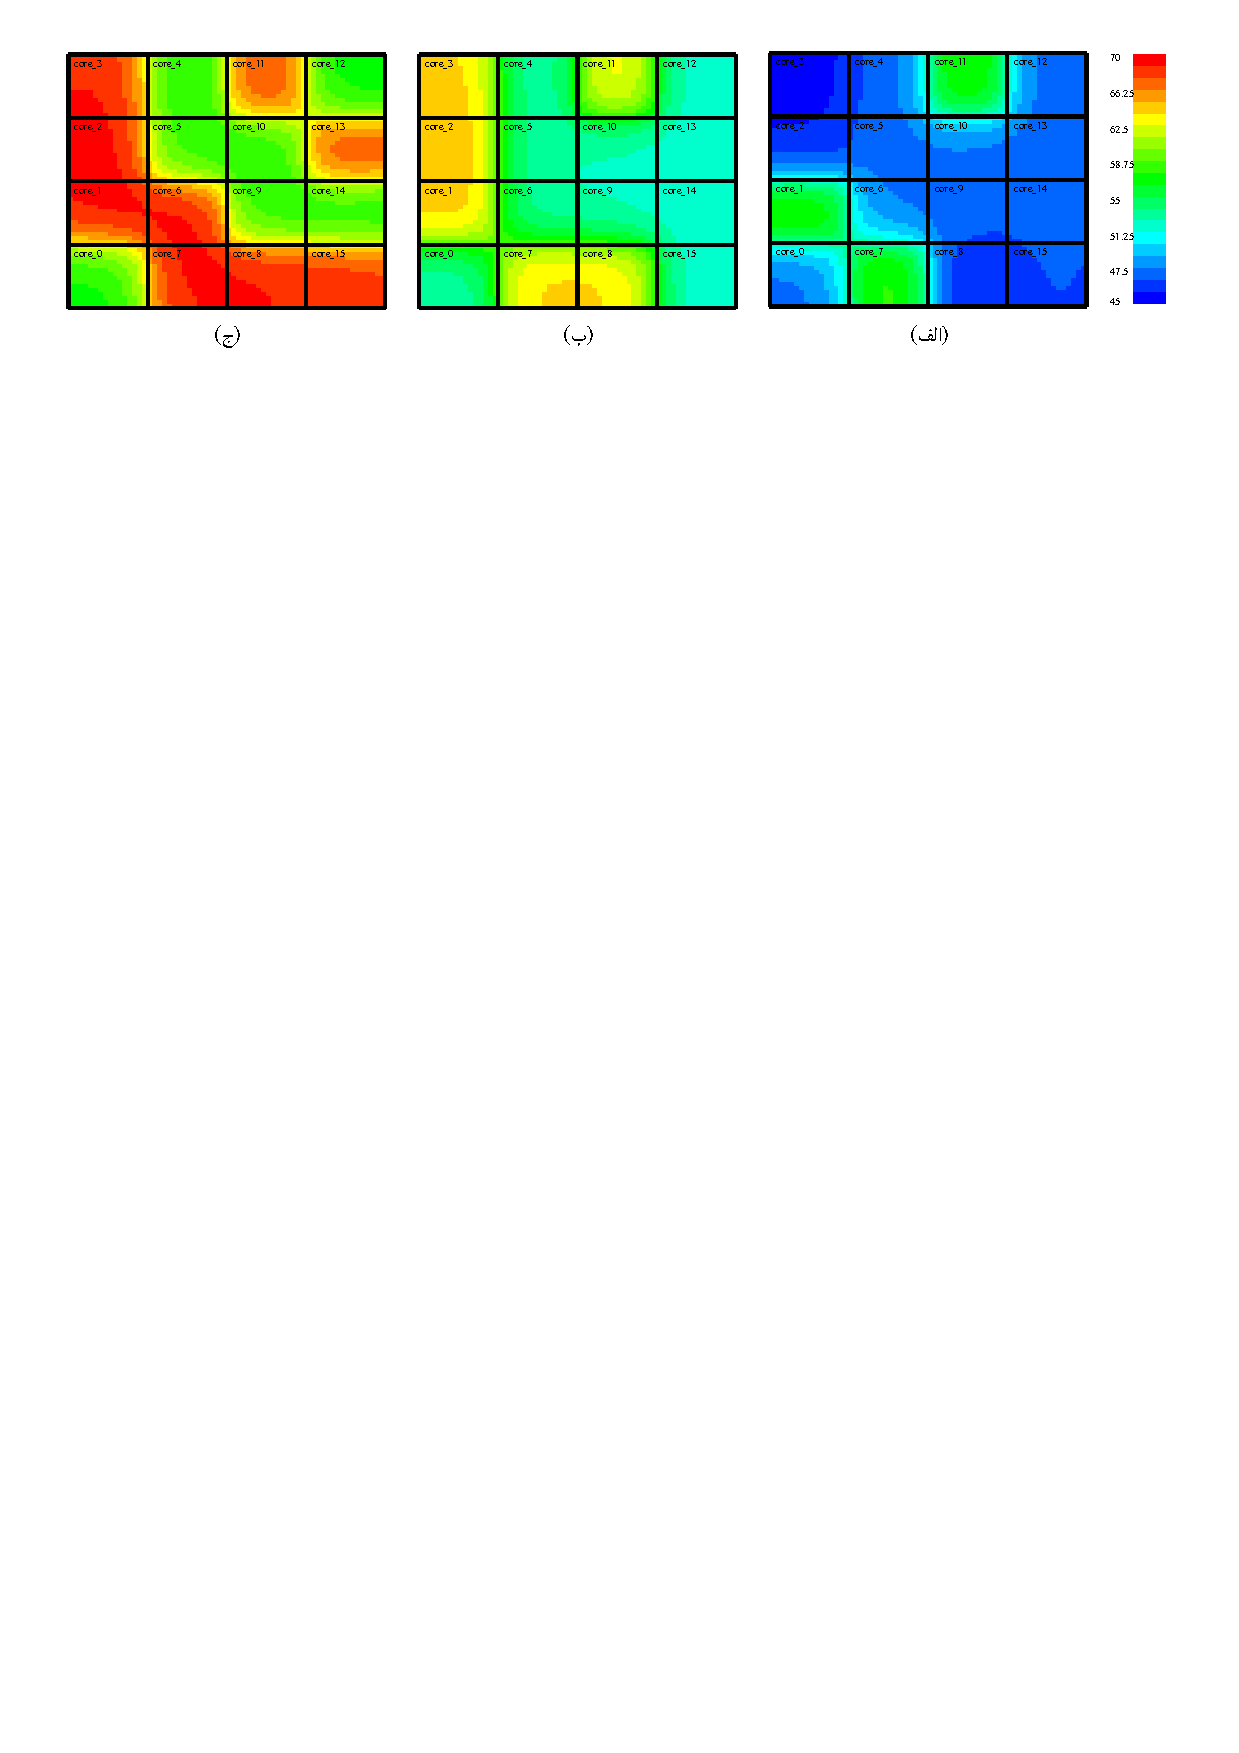
\includegraphics[scale=0.92]{images/ActiveCore.pdf}\\[0cm]
	\caption{بررسی تأثیر تعداد هسته‌های فعال بر دمای تراشه (الف) سه هسته‌ی فعال (ب) شش هسته‌ی فعال (ج) نه هسته‌ی فعال}
	\label{fig:ActiveCore}
\end{figure}

